\section{Results}
\label{sec:results}

We report two stages. An \emph{initial} threshold-crossing run on 12 healthy vs.\ 10 symptomatic necks
(Section~\ref{sec:res-initial}) established the headline canal/cord result and surfaced two leads
(disc and alignment). We then scaled and refined those two leads (Section~\ref{sec:res-scaled}); the
larger cohorts \emph{revised} both conclusions, and we report the revised, honest verdicts. This
progression --- not stopping at the encouraging small-sample numbers --- is itself a methodological
result.

\subsection{Initial run: canal/cord strong, compression null}
\label{sec:res-initial}
Table~\ref{tab:results} reports per-measure medians and the Mann--Whitney $U$ $p$-value on 12 healthy vs.\
10 symptomatic necks; Figure~\ref{fig:strips} shows the distributions.

\begin{table}[H]
\centering
\caption{Initial threshold-crossing run: healthy (12) vs.\ symptomatic MMCSD (10). The physical-dimension
(mm) metrics are scanner-immune and validate cross-dataset; the alignment and disc leads were
subsequently re-evaluated on larger cohorts (Section~\ref{sec:res-scaled}).}
\label{tab:results}
\begin{tabular}{l r r r l}
\toprule
\textbf{Measure} & \textbf{Healthy} & \textbf{Unhealthy} & \textbf{$p$} & \textbf{Verdict} \\
\midrule
G3 canal AP min (mm)      & 11.7 & 8.6 & \good{0.0001} & \good{strong separation} \\
G3 SAC min (mm)           & 4.7  & 2.3 & \good{0.0001} & \good{strong separation} \\
G3 cord AP min (mm)       & 6.3  & 5.5 & \good{0.009}  & \good{significant (thinner)} \\
G1 \hahp{} min            & 0.81 & 0.80& 0.92          & \good{correctly null (by design)} \\
G4 Cobb C1 C3--C7 (deg)   & 15.2 & 8.8 & 0.13          & lead --- re-evaluated below \\
G2 disc (DHI / bulge)     & --   & --  & --            & backwards (bug) --- root-caused, fixed below \\
\bottomrule
\end{tabular}
\end{table}

\begin{figure}[H]
\centering
\begin{subfigure}{0.32\textwidth}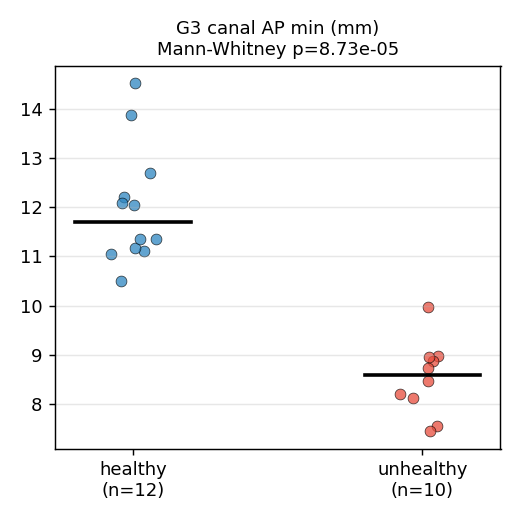
\includegraphics[width=\linewidth]{figures/canal-min.png}\caption{Canal AP min}\end{subfigure}\hfill
\begin{subfigure}{0.32\textwidth}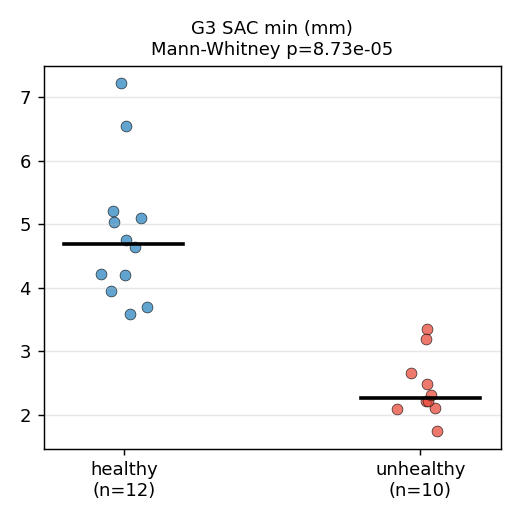
\includegraphics[width=\linewidth]{figures/sac-min.png}\caption{SAC min}\end{subfigure}\hfill
\begin{subfigure}{0.32\textwidth}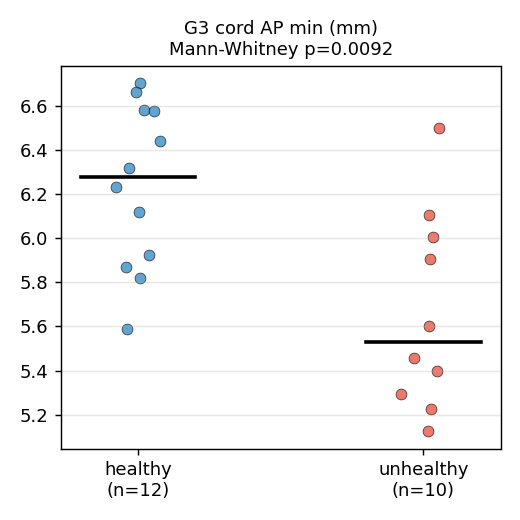
\includegraphics[width=\linewidth]{figures/cord-min.png}\caption{Cord AP min}\end{subfigure}
\caption{Initial-run healthy (blue) vs.\ unhealthy (red) distributions for the Group 3 physical-dimension
metrics; black bar is the median, with the Mann--Whitney $p$-value. Canal AP and SAC separate cleanly.}
\label{fig:strips}
\end{figure}

\subsection{Group 3 --- canal/cord/SAC: strong separation (the headline)}
Canal-AP minimum and SAC minimum both separate at $p=0.0001$; the distributions barely touch (healthy
canal floor \SI{10.5}{\milli\meter} vs.\ unhealthy ceiling \SI{9.97}{\milli\meter}). Cord AP is thinner in
the symptomatic cohort ($p=0.009$). On real MRI the canal/cord measurements read normal on healthy necks
and cross into stenosis on a CSM/CSR cohort --- the disease this cohort carries. Being physical-dimension
(mm) metrics, they are scanner-immune and validate cross-dataset.

\subsection{Group 1 --- compression: correctly null}
No difference (0.81 vs.\ 0.80, $p=0.92$), zero compression flags in either cohort --- the expected, correct
outcome: spondylosis is not compression fracture, so vertebral heights are normal (true negatives). This
empirically confirms the cohort does not exercise the compression axis (which needs a dedicated fracture
dataset) and re-confirms the Group 5.2 specificity on all 12 healthy controls.

\subsection{Scaled re-evaluation: the two leads, refined}
\label{sec:res-scaled}
The initial run left two leads --- a directional alignment signal and a (buggy) disc signal. We took both
to larger, design-appropriate cohorts. Crucially, the disc metrics are acquisition-sensitive
intensity/ratio quantities, so they must be validated \emph{within} one dataset, while alignment, though
geometric, carries a positioning confound across datasets.

\paragraph{Group 4 --- alignment: a validated \emph{method}, not a discriminator.}
The initial directional result (healthy \SI{+15.2}{\degree} vs.\ unhealthy \SI{+8.8}{\degree}, $p=0.13$,
$n{=}11$) did \emph{not} survive a representative sample. Adding multi-site healthy controls to reach
\textbf{26 healthy vs.\ 41 symptomatic} dropped the healthy mean to \SI{+10.7}{\degree} --- essentially
onto the symptomatic mean (\SI{+8.0}{\degree}) --- with \textbf{Cohen $d=0.28$, AUC $0.57$, $p=0.32$}: no
separation. The original $n{=}11$ was a \emph{lordosis-biased} draw (sites amu/beijingGE/fslAchieva, all
\SIrange{+13}{+21}{\degree}); the added sites are much flatter (nottwil \SI{+6}{\degree}, balgrist
\SI{+0.9}{\degree}, one healthy control \SI{-12.7}{\degree} kyphotic). Healthy cervical lordosis is simply
too variable (SD \(\sim\)\SI{10}{\degree}, range \SIrange{-13}{+32}{\degree}), and supine \emph{positioning}
is a cross-cohort confound. The endplate-voxel \emph{method} remains valid --- well-positioned controls
read \SIrange{+15}{+20}{\degree}, matching the standing-radiograph literature, with precise endplate fits
--- but cervical alignment is a biologically weak, non-specific marker of myelopathy. We therefore report
G4 as a validated \emph{measurement}, not a screen. Reporting the encouraging $n{=}11$ result as
``validated'' would have been a small-sample artifact; the larger sample caught it.

\paragraph{Group 2 --- disc: bugs fixed; geometric spread carries the only signal.}
The initial backwards reading was a real defect, since root-caused and corrected: vertebral heights were
measured by corner extrema (reading \hahp{} anterior-taller-than-posterior, \(\sim\)1.08, vs.\ the
physiological \(\sim\)0.94) and the disc bulge used corner-derived reference corners; switching both to the
validated endplate-line fit, and replacing a debunked absolute disc-height-index cut with a cited relative
($>$30\% cross-level) rule, removed the artifacts (healthy bulge over-flag $60\%\!\to\!8\%$). We then ran
the design-correct \emph{within-MMCSD} test (49 symptomatic cases, 276 disc-levels, lesion vs.\ non-lesion,
\emph{level-stratified} to remove the confound that lesions cluster at wider mid-cervical levels). The
disc \emph{signal} grade does not discriminate (AUC $0.50$, $p=0.93$) and neither does posterior bulge
(AUC $0.50$; TotalSpineSeg does not segment protrusion) --- two clean negatives. The discriminating
quantity is disc \emph{geometric spread}: the disc/vertebral-body AP-width ratio (AUC $0.62$, $p=0.0018$)
and disc AP width (AUC $0.61$ level-controlled; its raw AUC $0.79$ was mostly the level confound). Group~2
is therefore \emph{partially} validated --- a modest but honest geometric discriminator, with signal and
bulge documented as non-discriminators.

\subsection{Overall}
The validated-discriminator picture, after scaling, is clean and honest: \textbf{Group 3} (canal/SAC)
separates strongly ($p=0.0001$); \textbf{Group 2} disc/VB-AP-ratio separates modestly (AUC $0.62$);
\textbf{Group 4} alignment and the disc \emph{signal} axis are non-discriminators; \textbf{Groups 1 and 5}
are healthy-validated screens (with an under-tested compression arm). Four service-level measurement
defects (vertebral-height corner method, an over-aggressive tilt cut, the disc bulge reference, and a
debunked disc-height cut) were found and fixed during this work; the assessement layer (Group 6) was
wired end-to-end, including patient-demographic-aware thresholds. The recurring value is the methodology:
the harness doubled as a bug detector, level-stratification and a representative sample caught two
would-be false positives, and negative results were kept rather than buried.
